\documentclass[11pt,a4paper]{article}
\pdfmapfile{+lm.map}  % o updmap do Fedora vem com lm.map desativado
\usepackage[T1]{fontenc}
\usepackage[utf8]{inputenc}
\usepackage[brazilian]{babel}
\usepackage{lmodern,amsmath,booktabs,graphicx,xcolor}
\usepackage[expansion=false]{microtype}
\usepackage[margin=2.5cm]{geometry}
\usepackage[round,authoryear]{natbib}
\usepackage[hidelinks]{hyperref}

\newcommand{\todo}[1]{\textcolor{red}{[\textbf{A FAZER:} #1]}}
\newcommand{\ordo}{\textsuperscript{o}}
\newcommand{\anosAnalise}{2014, 2018, 2022}
\newcommand{\anoIni}{2014}
\newcommand{\anoFim}{2022}
\newcommand{\nAutovetores}{217}
\newcommand{\tUmA}{+0{,}2}
\newcommand{\tUmB}{+6{,}5}
\newcommand{\tDoisSalto}{5{,}2}
\newcommand{\tDoisLo}{3{,}5}
\newcommand{\tDoisHi}{6{,}7}
\newcommand{\tDoisPlacebo}{1{,}9}
\newcommand{\tDoisPlaceboLo}{0{,}8}
\newcommand{\tDoisPlaceboHi}{2{,}6}
\newcommand{\tDoisVeredito}{suportada}
\newcommand{\tDoisValidacao}{falhou: medida enviesada}
\newcommand{\eDoisEntre}{+3{,}4}
\newcommand{\eDoisDentro}{-3{,}4}
\newcommand{\eTresA}{+0{,}036}
\newcommand{\eTresB}{+0{,}060}
\newcommand{\tQuatroA}{deslocamento: religiosa}
\newcommand{\tQuatroB}{deslocamento: religiosa}
\newcommand{\tUmVA}{refutada}
\newcommand{\tUmVB}{suportada}
\newcommand{\eDoisVEntre}{estável ou caiu}
\newcommand{\eDoisVDentro}{estável ou caiu}
\newcommand{\eTresV}{misto: ver A e B}
\newif\ifparcial\parcialtrue
\newif\ifplacebook\placebookfalse
\newif\ifbymdois\bymdoisfalse


\title{Fé e fronteira: religião, território e a geografia\\
       do voto presidencial no Brasil (2014--2026)}
\author{\todo{nome e filiação}}
\date{Rascunho de \today}

\begin{document}
\maketitle

\ifparcial
\begin{center}\fbox{\parbox{0.9\linewidth}{\small\textbf{Versão parcial.}
Os resultados cobrem \anosAnalise. O pré-registro avalia as teses até 2026; todos os números,
tabelas e figuras serão recalculados com o mesmo código quando os arquivos definitivos do TSE para
2026 forem publicados. A interpretação abaixo é provisória.}}
\end{center}
\fi

\begin{abstract}
O mapa do voto presidencial brasileiro é um mapa de lugares ou de perfis sociais? Testamos teses
rivais, pré-registradas antes dos dados finais de 2026, sobre os 5.570 municípios em quatro
eleições presidenciais (2014--2026). Duas regularidades se destacam. Primeiro, o território
persiste: municípios socialmente parecidos e vizinhos votam diferente conforme o estado em que estão,
e o salto nas divisas estaduais é várias vezes maior que o de linhas arbitrárias traçadas dentro dos
estados. Segundo, a estrutura social que organiza o mapa mudou de natureza: a parcela do mapa que só a
religião explica, pequena em 2014, passou a ser de longe a maior entre as dimensões sociais em
2022, mais que o dobro da renda, nos dois campos políticos. Alinhando as séries por campo, o voto contra o PT foi o
que se reorganizou: em 2018 ele passou a seguir mais o perfil social dos municípios e menos o estado.
\ifparcial\todo{atualizar com o veredito final de 2026.}\fi
\end{abstract}

% ===========================================================================
\section{Introdução}

Desde 2006, o mapa do voto presidencial brasileiro tem uma forma reconhecível: o candidato do PT
vence com folga no Norte e no Nordeste, e seu principal adversário vence no Sul, no Centro-Oeste e
em boa parte do Sudeste \citep{soares2008,zucco2008,hunter2007}. Essa forma admite duas leituras.
Na primeira, o mapa é um retrato da composição social dos lugares: municípios mais pobres, menos
escolarizados ou mais católicos votam de um jeito, e a geografia é só a projeção dessas diferenças no
espaço. Na segunda, o lugar importa por si: estados têm elites, máquinas, imprensa e histórias
próprias, e dois municípios iguais em tudo, mas separados por uma divisa, votam diferente.

As duas leituras têm implicações distintas. Se o voto segue perfis, a polarização brasileira é uma
clivagem social que atravessa o território, como as clivagens de escolaridade e religião descritas
para outras democracias \citep{gethin2021}. Se segue lugares, ela é em parte uma clivagem
territorial, mais próxima da nacionalização incompleta dos sistemas partidários
\citep{jones2003} e da divisão entre cidades e interior \citep{rodden2019}. E, se segue perfis,
importa saber \emph{quais}: a literatura sobre 2018 aponta a religião como linha de divisão
crescente \citep{smith2019,layton2021}, enquanto a leitura clássica do realinhamento de 2006 enfatiza
renda e políticas sociais \citep{zucco2008,hunter2007}.

Este artigo confronta essas leituras com um desenho pré-registrado. Antes da divulgação dos dados
finais de 2026, fixamos publicamente as teses, as medidas e os limiares que decidem entre elas
\citep{nosek2018}. Analisamos os 5.570 municípios em quatro eleições, com três estratégias: (i) uma
decomposição de Shapley que reparte o mapa entre estrutura social, vizinhança e estado; (ii) uma
comparação de municípios vizinhos separados por divisas estaduais, contra uma distribuição de linhas
arbitrárias; e (iii) uma decomposição da estrutura social em cinco dimensões censitárias.

Os resultados sustentam uma síntese que chamamos de \emph{fé e fronteira}. O território não
desapareceu: o salto nas divisas estaduais, condicionado ao perfil social, é de \dado{real\anoFim} p.p.
em \anoFim{}, e nenhuma das \dado{nPlacebos} linhas arbitrárias chega perto disso. Ao mesmo tempo, a
estrutura que organiza o mapa mudou: a religião, e não a renda, passou a ser a dimensão social com
maior poder explicativo próprio. A mudança foi assimétrica no tempo: em 2018, o voto contra o PT se
desprendeu dos estados e passou a seguir o perfil social dos municípios; em 2022, a religião se
tornou a principal linha de separação dos dois lados.

O artigo contribui de três formas. Substantivamente, mostra que a polarização brasileira combina uma
clivagem religiosa nacional com uma clivagem territorial persistente, e não uma substituindo a outra.
Metodologicamente, propõe uma medida do salto nas divisas sem o viés de ruído das medidas usuais e a
compara com uma distribuição de linhas-placebo. E, em termos de transparência, separa explicitamente
o que foi testado como pré-registrado do que foi descoberto depois, uma distinção rara na geografia
eleitoral.

% ===========================================================================
\section{Lugares ou perfis: expectativas}

\todo{revisão de literatura em 2 ou 3 parágrafos: geografia eleitoral brasileira (Soares e Terron;
Zucco; Hunter e Power; Limongi e Guarnieri); religião e voto (Smith; Layton et al.); clivagens
comparadas (Gethin, Martínez-Toledano e Piketty); nacionalização (Jones e Mainwaring). Conferir cada
referência antes de citar.}

As expectativas pré-registradas se organizam em quatro eixos. No \textbf{eixo 1}, a tese da
\emph{estruturação} (T1) prevê que a parcela do mapa explicada pela estrutura social cresceu, e a do
estado caiu; a tese do \emph{território persistente} (T2) prevê que o salto nas divisas estaduais é
grande e não diminuiu. No \textbf{eixo 4}, a tese da \emph{renda} prevê que a dimensão econômica é a
que mais separa os municípios; a do \emph{deslocamento}, que outra dimensão (escolaridade ou religião)
a ultrapassou. Os eixos 2 (onde está a variância: entre ou dentro dos municípios) e 3 (isolamento
entre os blocos) completam o desenho e são resumidos na Seção~\ref{sec:eixos23}.

% ===========================================================================
\section{Dados e desenho}

\paragraph{Unidades e desfechos.} Os 5.570 municípios, com votos do TSE nos dois turnos de 2014,
2018 e 2022 \ifparcial (2026 entra quando os arquivos definitivos forem publicados)\fi. Os
desfechos são as participações dos dois primeiros colocados nos votos válidos do 1\ordo{} turno, em
logit. Boa Esperança do Norte (MT), criado depois de 2022, é agregado a seus municípios de origem.

\paragraph{Blocos.} O pré-registro define os blocos por posição (A: primeiro colocado nacional no
1\ordo{} turno; B: segundo), para não depender de nomes ou partidos. Essa escolha tem um custo: o bloco
A é o PT em 2014 e 2022, mas o adversário do PT em 2018, e uma tendência do bloco A mistura lados.
Como o PT esteve entre os dois primeiros nas quatro eleições, as análises exploratórias alinham as
séries por campo: \emph{PT} e \emph{adversário} (o outro entre os dois primeiros). O alinhamento não
envolve escolha do pesquisador.

\paragraph{Estrutura social.} Cinco dimensões, com definição idêntica nos Censos de 2010 (usado em
2014 e 2018) e 2022: econômica (\% de moradores com renda \emph{per capita} até meio salário mínimo),
educacional (\% com superior completo, 25 anos ou mais), religiosa (\% de evangélicos, católicos e
sem religião), demográfica (\% urbana, log do eleitorado) e cor/raça (\% de pretos e pardos, \% de
indígenas).

\paragraph{Decomposição do mapa.} Para cada eleição e bloco, um MQO ponderado pelo eleitorado sobre
três grupos de regressores: estrutura social, vizinhança e estado (efeitos fixos de UF). A vizinhança
é um filtro espacial de autovetores \citep{griffith2003,tiefelsdorf2007} do grafo de contiguidade,
com \nAutovetores{} autovetores. O $R^2$ ajustado é repartido entre os três grupos pelo valor de
Shapley \citep{gromping2006}. A mesma decomposição, aplicada às cinco dimensões dentro da estrutura,
dá a \emph{parcela única} de cada dimensão: quanto o $R^2$ cai quando só ela é retirada. A parcela
compartilhada, grande porque renda, escolaridade e cor/raça andam juntas, não é atribuída a nenhuma.
Os intervalos de 90\% vêm de 200 réplicas de \emph{bootstrap} de municípios estratificado por UF.

\paragraph{Salto nas divisas.} Em pares de municípios contíguos separados por divisa estadual
\citep{keele2015}, a diferença de voto dentro do par é regredida nas diferenças de estrutura e nos
efeitos de UF. O salto típico é o desvio quadrático médio entre os efeitos estimados das duas UFs
de cada par, descontada a variância exata do estimador:
\begin{equation}
  J = \sqrt{\overline{(\hat\gamma_a - \hat\gamma_b)^2} - \overline{\operatorname{Var}(\hat\gamma_a - \hat\gamma_b)}}.
\end{equation}
Sem o desconto, o ruído municipal inflaria qualquer salto estimado. Para saber se $J$ é grande, a
mesma medida é calculada em linhas-placebo que partem cada estado ao meio; o pré-registro usa uma
linha (a mediana da longitude), e a análise exploratória usa \dado{nPlacebos} linhas com direção e
posição sorteadas.

% ===========================================================================
\section{Resultados pré-registrados}\label{sec:prereg}

\ifparcial\noindent\emph{Parciais: \anosAnalise.}\par\fi
A Tabela~\ref{tab:veredito} aplica mecanicamente as regras do pré-registro.

\begin{table}[htbp]\centering\small
\caption{Vereditos pelas regras pré-registradas (blocos posicionais).}\label{tab:veredito}
\begin{tabular}{llrrr}
\toprule
Tese & Veredito & Estimativa & IC90\% inf. & IC90\% sup. \\
\midrule
T1 estruturação (bloco A) & refutada & +0{,}002 & -0{,}009 & +0{,}013 \\
T1 estruturação (bloco B) & suportada & +0{,}065 & +0{,}050 & +0{,}082 \\
T2 território (salto corrigido, p.p.) & suportada & +5{,}243 & +3{,}514 & +6{,}695 \\
T2 placebo (validação) & falhou: medida enviesada & +1{,}906 & +0{,}833 & +2{,}595 \\
Eixo 2 entre lugares ($\Delta$ parcela) & estável ou caiu & +0{,}034 & +0{,}016 & +0{,}053 \\
Eixo 2 dentro dos lugares ($\Delta$ parcela) & estável ou caiu & -0{,}034 & -0{,}053 & -0{,}016 \\
Eixo 3 $\Delta$ isolamento A (local) &  & +0{,}036 & +0{,}027 & +0{,}044 \\
Eixo 3 $\Delta$ isolamento B (local) &  & +0{,}060 & +0{,}038 & +0{,}075 \\
Eixo 3 veredito & misto: ver A e B &  &  &  \\
T4 (bloco A) & deslocamento: religiosa &  &  &  \\
T4 (bloco B) & deslocamento: religiosa &  &  &  \\
\bottomrule
\end{tabular}

\end{table}

\paragraph{T1 (estruturação).} A tendência da parcela estrutural foi de \tUmA{} p.p. no bloco A
(\emph{\tUmVA}) e de \tUmB{} p.p. no bloco B (\emph{\tUmVB}). Como os blocos posicionais trocam de
lado em 2018, esse contraste é difícil de interpretar diretamente; a Seção~\ref{sec:explor} mostra o
que ele esconde.

\paragraph{T2 (território).} O salto nas divisas em \anoFim{} foi de \tDoisSalto{} p.p. (IC90\%
\tDoisLo{} a \tDoisHi{}; veredito: \emph{\tDoisVeredito}). Na linha-placebo do pré-registro, a mesma
medida deu \tDoisPlacebo{} p.p. (IC90\% \tDoisPlaceboLo{} a \tDoisPlaceboHi{}).
\ifplacebook
O intervalo do placebo contém zero, como exigido.
\else
A regra pré-registrada exige que esse intervalo contenha zero, e ele não contém: a validação falhou.
Reportamos o veredito ao lado da falha, sem alterar a medida. A Seção~\ref{sec:explor} sugere a razão:
uma única linha de longitude corta regiões genuinamente diferentes dentro de alguns estados, de modo
que o placebo mede diferenças regionais reais, e não apenas viés.
\fi

\paragraph{T4 (qual diferença divide).} O veredito é \emph{\tQuatroA} no bloco A e \emph{\tQuatroB}
no bloco B (Tabela~\ref{tab:eixo4}). Esse é o resultado mais robusto do desenho: ele não depende do
alinhamento dos blocos.

% ===========================================================================
\section{Fé e fronteira: análises exploratórias}\label{sec:explor}

\noindent\emph{As análises desta seção foram definidas depois de ver os resultados parciais e não
fazem parte do pré-registro.}

\subsection{O voto contra o PT se reorganizou em 2018}

A Figura~\ref{fig:shapley} alinha a decomposição por campo. No PT, as parcelas são estáveis: a
estrutura social explica \dado{estPT\anoIni} do $R^2$ em \anoIni{} e \dado{estPT\anoFim} em
\anoFim{}. No adversário, a estrutura sobe de \dado{estAdv2014} em 2014 para \dado{estAdv2018} em
2018, e o estado cai de \dado{ufAdv2014} para \dado{ufAdv2018}. O voto contra o PT, que em 2014 ainda
variava muito de estado para estado, passou a seguir o perfil social dos municípios de forma quase
uniforme no país. O contraste posicional da Tabela~\ref{tab:veredito} (T1 suportada só para B) é a
sombra desse movimento: em 2018, o bloco B é o PT, e a série posicional mistura os dois lados.

\begin{figure}[htbp]\centering
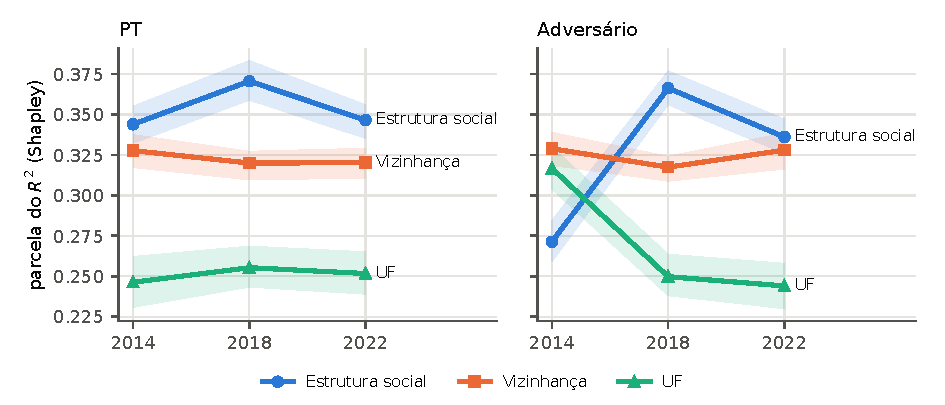
\includegraphics[width=\linewidth]{figuras/fig_shapley}
\caption{Parcelas de Shapley do $R^2$ ajustado, alinhadas por campo. Linhas: mediana do
\emph{bootstrap}; faixas: IC90\%. As estimativas pontuais ficam cerca de 0,01 acima das medianas em
todos os anos (Tabela~\ref{tab:eixo1}), o que não altera as tendências.}\label{fig:shapley}
\end{figure}

\subsection{A religião passou a renda}

A Figura~\ref{fig:dimensoes} decompõe a estrutura. Em 2014, a parcela única da religião era pequena
nos dois campos (\dado{relPT2014} no PT, já um pouco acima da renda, e \dado{relAdv2014} no
adversário, bem abaixo dela). Em \anoFim{}, ela é a
maior entre as cinco dimensões: \dado{relPT\anoFim} no PT e \dado{relAdv\anoFim} no adversário,
contra \dado{rendaPT\anoFim} e \dado{rendaAdv\anoFim} da renda. No adversário, o crescimento já
aparece em 2018 (\dado{relAdv2018}); no PT, ele se concentra em 2022. A escolaridade, apontada como
a clivagem emergente em outras democracias \citep{gethin2021}, tem parcela única próxima de zero em
todos os anos: o que ela explica, explica junto com renda e cor/raça.

\begin{figure}[htbp]\centering
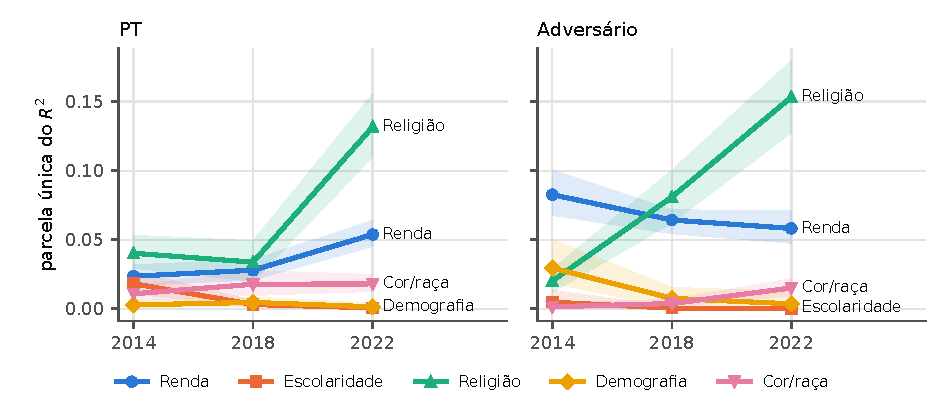
\includegraphics[width=\linewidth]{figuras/fig_dimensoes}
\caption{Parcela única de cada dimensão social no $R^2$ (quanto o ajuste cai quando só ela é
retirada), alinhada por campo. Mediana e IC90\% do \emph{bootstrap}.}\label{fig:dimensoes}
\end{figure}

\ifexploratorio
A Figura~\ref{fig:coef} mostra quais variáveis carregam o efeito. \todo{descrever depois de ver os
coeficientes: sinal e evolução de \% evangélicos (\dado{ev\anoIni} em \anoIni, \dado{ev\anoFim} em
\anoFim), \% católicos e \% sem religião, comparados à renda.}

\begin{figure}[htbp]\centering
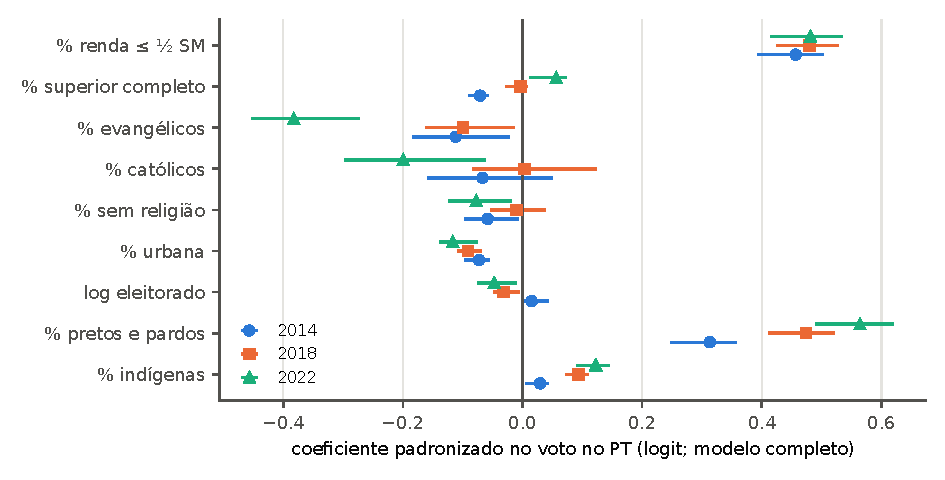
\includegraphics[width=\linewidth]{figuras/fig_coeficientes}
\caption{Coeficientes padronizados no voto no PT (logit), no modelo com estrutura, vizinhança e
efeitos de UF. Pontos: estimativa; barras: IC90\% do \emph{bootstrap}.}\label{fig:coef}
\end{figure}
\fi

\subsection{A fronteira persiste}

\ifexploratorio
A Figura~\ref{fig:fronteira} compara o salto nas divisas estaduais com o de \dado{nPlacebos} linhas
traçadas ao acaso dentro dos estados. Em \anoFim{}, a mediana das linhas-placebo é \dado{plMed\anoFim}
p.p., e a maior delas chega a \dado{plMax\anoFim} p.p.; nas divisas reais, o salto é de
\dado{real\anoFim} p.p. (linhas-placebo com salto igual ou maior: \dado{plAcima\anoFim}). O padrão se
repete nos três anos. As divisas estaduais não são uma descontinuidade espacial qualquer: elas
separam municípios parecidos que votam diferente.

\begin{figure}[htbp]\centering
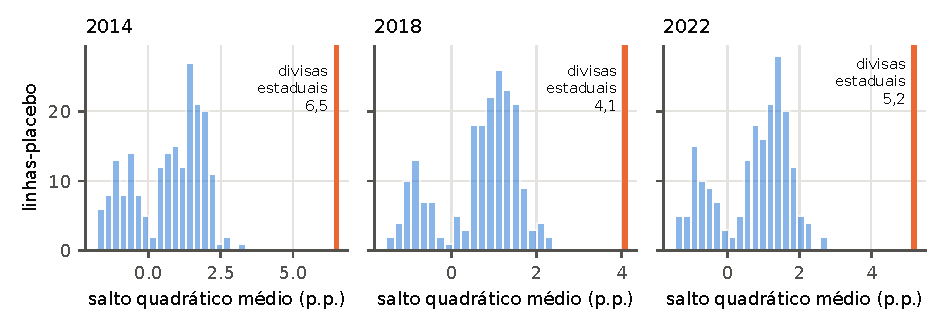
\includegraphics[width=\linewidth]{figuras/fig_fronteira}
\caption{Salto quadrático médio nas divisas estaduais (linha) e em \dado{nPlacebos} linhas-placebo
com direção e posição sorteadas dentro de cada estado (histograma), condicionado à estrutura
social.}\label{fig:fronteira}
\end{figure}

A Figura~\ref{fig:mapa} mostra onde está o território: o efeito de cada estado no voto no PT, depois
de descontado o perfil social de seus municípios.
\todo{descrever o mapa: quais estados votam acima ou abaixo do esperado pelo perfil social.}

\begin{figure}[htbp]\centering
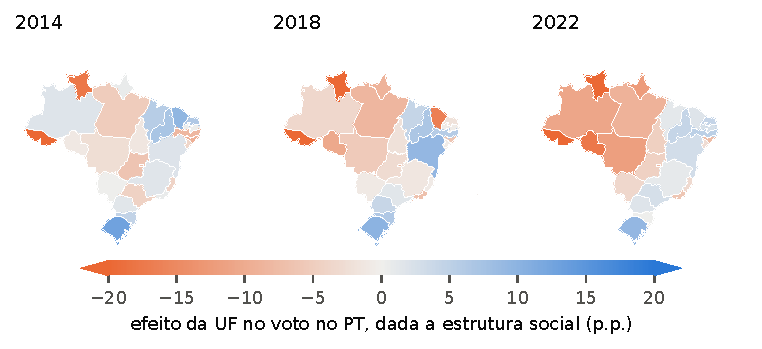
\includegraphics[width=\linewidth]{figuras/fig_mapa_uf}
\caption{Efeito de cada UF no voto no PT (p.p.), num MQO ponderado com a estrutura social, centrado
na média nacional.}\label{fig:mapa}
\end{figure}
\else
\todo{distribuição de linhas-placebo e mapa dos efeitos de UF (\texttt{geovoto.teses\_extra}).}
\fi

% ===========================================================================
\section{Onde está a divisão e quem convive com quem}\label{sec:eixos23}

Os eixos 2 e 3 do pré-registro dão o contexto. A variância do voto entre os dois blocos está
concentrada entre estados e entre municípios; a parcela entre lugares variou \eDoisEntre{} p.p. no
período (\emph{\eDoisVEntre}) e a parcela dentro dos municípios, entre locais de votação,
\eDoisDentro{} p.p. (\emph{\eDoisVDentro}; Tabela~\ref{tab:eixo2}). No local de votação, o
isolamento variou \eTresA{} no bloco A e \eTresB{} no bloco B (veredito: \emph{\eTresV};
Tabela~\ref{tab:eixo3}).

% ===========================================================================
\section{Discussão}

\ifparcial\noindent\emph{Provisória, sobre \anosAnalise.}\par\fi
O mapa eleitoral brasileiro não escolheu entre lugares e perfis. Ele combina uma clivagem religiosa
que atravessa o país, crescente e já maior que a de renda, com uma clivagem territorial que as
divisas estaduais ainda marcam com nitidez. As duas coisas são compatíveis porque a estrutura social
explica a \emph{inclinação} do voto dentro de cada estado, enquanto o estado desloca o \emph{nível}.

Três cautelas. Primeiro, as afirmações valem para lugares, não para pessoas \citep{robinson1950}:
``municípios mais evangélicos'' não equivale a ``eleitores evangélicos''. A validação com dados
individuais do Estudo Eleitoral Brasileiro é o próximo passo. Segundo, as variáveis religiosas de 2014
e 2018 vêm do Censo de 2010; parte do crescimento da parcela religiosa em 2022 pode refletir a
atualização para o Censo de 2022. Terceiro, a análise alinhada por campo e a distribuição de
placebos são exploratórias. \ifparcial Os dados de 2026 são o teste fora da amostra dessas
regularidades.\fi
\todo{conferir a cautela do Censo: refazer 2022 com o Censo 2010 como robustez.}

% ===========================================================================
\section{Limitações}

Falácia ecológica \citep{robinson1950}; dependência de escala \citep{openshaw1984}, tratada com três
níveis no eixo 2 e com regiões imediatas no lugar de UF na robustez; a ``vizinhança'' é dependência
residual, não contágio; covariáveis censitárias defasadas em relação a 2018 e 2026; o
\emph{bootstrap} das parcelas de Shapley fica cerca de 0,01 abaixo das estimativas pontuais.
\ifplacebook\else A validação por placebo do T2 falhou nos dados reais (Seção~\ref{sec:prereg}).\fi

% ===========================================================================
\appendix
\section{Tabelas}

\begin{table}[htbp]\centering\small
\caption{Decomposição de Shapley do $R^2$ ajustado (eixo 1, blocos posicionais, estimativas pontuais).}\label{tab:eixo1}
\begin{tabular}{llrrrrr}
\toprule
Ano & Bloco & Estrutura & Vizinhança & UF & Compartilhado & $R^2_{aj}$ \\
\midrule
2014 & A & 0{,}356 & 0{,}312 & 0{,}241 & 0{,}721 & 0{,}909 \\
2014 & B & 0{,}275 & 0{,}317 & 0{,}317 & 0{,}742 & 0{,}908 \\
2018 & A & 0{,}377 & 0{,}304 & 0{,}245 & 0{,}749 & 0{,}927 \\
2018 & B & 0{,}384 & 0{,}305 & 0{,}250 & 0{,}751 & 0{,}940 \\
2022 & A & 0{,}356 & 0{,}306 & 0{,}247 & 0{,}726 & 0{,}908 \\
2022 & B & 0{,}344 & 0{,}314 & 0{,}239 & 0{,}710 & 0{,}897 \\
\bottomrule
\end{tabular}

\end{table}

\begin{table}[htbp]\centering\small
\caption{Salto nas divisas estaduais e na linha-placebo do pré-registro (p.p.; mediana e IC90\% do \emph{bootstrap}).}\label{tab:fronteira}
\begin{tabular}{lrcrc}
\toprule
Ano & Divisas reais & IC90\% & Placebo & IC90\% \\
\midrule
2014 & 6{,}32 & [4{,}87; 8{,}05] & 2{,}18 & [-0{,}75; 3{,}13] \\
2018 & 4{,}26 & [2{,}91; 5{,}55] & 1{,}51 & [0{,}24; 2{,}29] \\
2022 & 5{,}24 & [3{,}51; 6{,}70] & 1{,}91 & [0{,}83; 2{,}59] \\
\bottomrule
\end{tabular}

\end{table}

\begin{table}[htbp]\centering\small
\caption{Efeitos únicos das dimensões estruturais (eixo 4, blocos posicionais).}\label{tab:eixo4}
\resizebox{\linewidth}{!}{\begin{tabular}{llrrrrrr}
\toprule
Ano & Bloco & Econômica & Educacional & Religiosa & Demográfica & Cor/raça & Compart. \\
\midrule
2014 & A & 0{,}024 & 0{,}017 & 0{,}040 & 0{,}002 & 0{,}011 & 0{,}671 \\
2014 & B & 0{,}083 & 0{,}004 & 0{,}020 & 0{,}029 & 0{,}001 & 0{,}525 \\
2018 & A & 0{,}064 & 0{,}000 & 0{,}082 & 0{,}007 & 0{,}003 & 0{,}658 \\
2018 & B & 0{,}029 & 0{,}003 & 0{,}034 & 0{,}004 & 0{,}017 & 0{,}721 \\
2022 & A & 0{,}054 & 0{,}001 & 0{,}133 & 0{,}001 & 0{,}018 & 0{,}572 \\
2022 & B & 0{,}058 & 0{,}000 & 0{,}155 & 0{,}003 & 0{,}014 & 0{,}517 \\
\bottomrule
\end{tabular}
}
\end{table}

\begin{table}[htbp]\centering\small
\caption{Parcelas da variância de $\operatorname{logit}(A/(A+B))$ por nível (eixo 2).}\label{tab:eixo2}
\begin{tabular}{lrrrr}
\toprule
Ano & UF & Município & Local de votação & Variância total \\
\midrule
2014 & 0{,}582 & 0{,}201 & 0{,}217 & 1{,}415 \\
2018 & 0{,}536 & 0{,}285 & 0{,}179 & 1{,}755 \\
2022 & 0{,}506 & 0{,}310 & 0{,}183 & 0{,}722 \\
\bottomrule
\end{tabular}

\end{table}

\begin{table}[htbp]\centering\small
\caption{Isolamento e exposição (eixo 3).}\label{tab:eixo3}
\begin{tabular}{llrrrr}
\toprule
Ano & Escala & Isol. A & Isol. B & Expos. A$\to$B & Expos. B$\to$A \\
\midrule
2014 & Município & 0{,}492 & 0{,}406 & 0{,}286 & 0{,}356 \\
2014 & Local & 0{,}509 & 0{,}429 & 0{,}271 & 0{,}337 \\
2018 & Município & 0{,}521 & 0{,}420 & 0{,}230 & 0{,}361 \\
2018 & Local & 0{,}530 & 0{,}443 & 0{,}219 & 0{,}345 \\
2022 & Município & 0{,}534 & 0{,}480 & 0{,}387 & 0{,}434 \\
2022 & Local & 0{,}544 & 0{,}489 & 0{,}378 & 0{,}424 \\
\bottomrule
\end{tabular}

\end{table}

\section{Robustez}

\ifbymdois
\begin{table}[htbp]\centering\small
\caption{Diagnósticos de convergência do BYM2 \citep{riebler2016}.}\label{tab:bym2}
% BYM2 ainda não rodou

\end{table}
\todo{coeficientes do BYM2 versus MQO.}
\else
\todo{BYM2 \citep{riebler2016} em execução.}
\fi
\todo{sensibilidade do filtro espacial (limiares 0,5 e 0,25), regiões imediatas e 2\ordo{} turno.}

\section{Desvios do pré-registro}

\begin{enumerate}
  \item O veredito calculado sem 2026 recebe o rótulo ``parcial''.
  \item O BYM2 passou a usar o amostrador NUTS do \texttt{nutpie}, porque o padrão do PyMC não
        terminou nenhum modelo em 4 horas.
  \item No primeiro ajuste, o BYM2 não convergiu no intercepto ($\hat R = 1{,}18$), que não é
        identificado separadamente da média dos efeitos de UF. Os efeitos de UF passaram a ter soma
        zero (reparametrização) e as amostras por cadeia subiram de 1.000 para 2.000.
  \item As análises da Seção~\ref{sec:explor} são exploratórias e foram definidas depois dos resultados
        parciais.
\end{enumerate}

\bibliographystyle{abbrvnat}
\bibliography{referencias}
\end{document}
